%# -*- coding: utf-8-unix -*-
%%==================================================
%% chapter01.tex for SJTU Master Thesis
%%==================================================

\chapter{绪论}
\label{chap:overview}



\section{引言}
\label{sec:introduction}
据统计,截止2015年上半年,中国电影3D银幕数量已占全国银幕总数的70\%之多,这标志着中国电影已正式进入3D时代。于此同时,目前市场在售的高清电视机基本都支持3D显示,3D应用越来越广泛。与2D资源类似,立体图像(视频)在应用过程中也要经过编码、传输、存储、解码等过程,这些环节都可能产生图像的失真。因此,在立体图像应用过程中图像质量的测评机制就显得很重要\parencite{galkandage2015full}。和2D图像一样,立体图像质量评价方法有主观评价和客观评价之分,受限于高昂的时间和人力成本,主观评价并不适用于工业生产领域,这使得基于图像自身特征的客观质量评价方法在计算机速率迅速提高的背景下得到了广泛应用,因此,提升客观图像质量评价方法的性能至关重要。而客观质量评价方法的效果则需要以主观评价结果来衡量,所以,主客观图像质量评价方法的结合是科研领域的重要方法之一。

近年来立体图像质量评价方法开始从直接的图像特征提取向引入人眼视觉特征转变\parencite{bensalma2013perceptual,engelke2011visual,hachicha2013stereo,ryu2014no}。引入视觉特征的其中一个方法就是利用眼动仪来标记用户的注视区域,从而用注视区域的特征取代整体图像的特征\parencite{ninassi2007does}。这种方法很好地提升了现有的基于图像特征的立体图像质量评价方法的效果\parencite{liu2009studying,liu2011visual}。但是,这些研究方法并没有考虑眼动数据自身的特征,作为眼睛运动过程的记录,眼动数据本身的特征并没有受到重视。因此,本文将研究眼动数据自身的特征与立体图像质量之间的关系。

\section{论文研究的背景及意义}
\label{sec:background}
图像质量评价的过程是视觉系统对看到的图像进行处理后得到的好恶判断的过程。眼睛注视到图像后,其接收到的信息进入视觉系统,大脑皮层对图像进行特征提取、编码,最后在中枢神经系统进行融合、成像\parencite{zhu20143d}。由于人眼视觉系统经过长时间的进化,对所见事物有经验的积累,当大脑皮层重构出所看事物的像后,大脑会从主观上将看到的图像与积累的经验进行对比,从而对图像做出优劣判断\parencite{liu2010scene},这个过程可以以图\ref{fig:pycologyprocess}来表示。因此,起初的图像质量评价具有经验性的特点。随着工业科技的发展,人们在工程实践中发现亮度、色度、纹理等特征是影响图像质量的重要因素,所以,图像质量评价的方法转向图像特征的提取上,这种转变在现代计算机性能逐步提高的背景下很有意义,一系列基于整体图像特征的客观评价方法被提了出来,如PSNR,SSIM\parencite{wang2003multiscale},BLIINDS-II\parencite{saad2012blind}以及基于梯度相似性的IQA\parencite{liu2012image}等,这些算法在2D图像质量评价中发挥了重要的作用。
\begin{figure}[!htp]
  \centering
  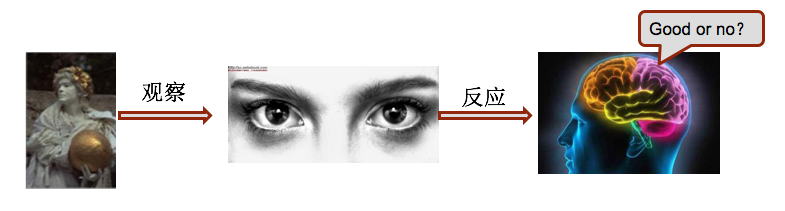
\includegraphics[width=0.8\textwidth]{chap1/pycologyprocess.png}
  \bicaption[fig:pycologyprocess]{图像质量评价的生理过程}{图像质量评价的生理过程}{Fig}{The physiological process of image quality assessment}
\end{figure}

近些年基础科学研究的成果为基于特征的图像质量评价方法奠定了生理学基础。研究表明,图像特征与图像质量关联的原因是视觉系统中存在着处理这些特征的神经与细胞\parencite{hubel1962receptive},更近一步的,人们还发现了大脑皮层处理图像特征的方式与方法\parencite{barlow1967neural,fleet1996neural},这些将在第\ref{chap:humanview}章进行详细描述。这些成果从两方面影响了图像质量评价的发展:一方面是人们意识到影响图像质量的并不是图像的整体,而是进入视觉系统的部分,因此,图像特征的提取从整体转向了局部;另一方面是,大脑皮层处理图像的生理过程越来越明了,使得在图像质量评价中模拟人类视觉系统成为一种可能。因此,近年来,基于人眼注视特征的图像质量评价方法越来越多\parencite{wang2002no,zhang2011fsim,wang2004video,chen2006gradient}。眼动数据在这类模型中发挥了重要的作用\parencite{fliegel2008eyetracking,gide2012comparative},特别是2D图像质量评价中,利用眼动数据作为groundtruth标记的注视区域,有效的提升了基于特征的图像质量评价方法的效果\parencite{gidevisual,meining2010eye}。正因如此,近年来研究人员开始将眼动数据引入立体图像质量评价中。

相比较2D图像质量评价,眼动数据在立体图像质量评价中可以发挥更大的作用,其理由有三:第一,传统的2D图像质量评价方法在3D图像质量评价中的效果并不太好\parencite{bensalma2013perceptual},而基于人眼注视模型的图像质量评价是目前该领域研究的重点;第二,影响3D图像质量最重要的因素之一是视差,视差涉及双目视觉过程,眼动数据可以记录眼睛的运动过程,可以描述双目视觉的变化过程;第三,观看2D图像时,由于聚焦在屏幕上,眼动数据往往关注两只眼睛的综合功能,而观看3D图像时,两只眼睛看到的是“不同”的画面,此时的眼动数据很有可能描绘这种“不同”。

但是,目前眼动数据在3D图像质量评价中的应用受到了限制,常见的用法还是停留在标记显著性区域,创建人眼注视区域的groundtruth等。造成这种现象的原因比较多。第一,眼动数据在2D图像质量评价中的应用方法已经被证明是有用的\parencite{gidevisual,meining2010eye},因此,直接采用这样的方法的效果是可以保障的;第二,2D图像质量评价经过了长时间的发展,形成了成熟的评价体系,包括研究方法和研究图库等,因此,基于这些图库建立了较完备的眼动数据集\parencite{winkler2013overview}。而3D图像的整体研究水平并没有到达这样的层次\parencite{bensalma2013perceptual},这无疑限制了眼动数据在该领域的应用;第三,3D下眼动数据的处理技术不完备,目前的眼动数据的滤波、校正、表示等基础技术,基本还是2D场景下处理技术的延续;第四,受限于当前眼动仪的精度,眼动数据标记注视区域时误差精度可忍受,但涉及到视差角等更精细的特征时,其误差较大,这使得当前很少有研究关注眼动数据本身的特征。

从目前已有的研究成果中我们可以发现,眼动数据在已有的2D图像质量评价方法中的效果已经被肯定,但是受限于当前3D领域研究基础比较薄弱与相关的眼动技术无法达到3D特征描述的精度,使眼动仪在3D图像质量评价中的应用受到了限制。其次,作为眼动过程的记录,眼动数据的注视区域特征与图像质量的关联也得到了证实。基于上述分析,我们尝试着来验证眼动数据特征与立体图像质量之间是否存在关联。本文具体的工作从以下三个方面展开:
\begin{itemize}[noitemsep,topsep=0pt,parsep=0pt,partopsep=0pt]
\item 建立立体图像-眼动数据库,为眼动数据特征提取做好准备;
\item 对比分析2D与3D场景下眼动数据基础技术的区别,结合前人的研究算法,给出3D场景下眼动数据的滤波、校正以及表示等方法,并分析其结果;
\item 针对创建的立体图像-眼动数据库,结合上述的眼动数据的处理技术,提取眼动数据特征,并与MOS值进行SVR拟合,讨论利用眼动数据特征评价立体图像质量的可行性。
\end{itemize}

期望通过本问题的研究,可以在创建数据集、基础研究方法等领域做出些许贡献,最重要的是,通过论证眼动数据自身在立体图像质量评价中的作用,拓宽眼动数据的应用领域。

\section{国内外研究现状}
\label{sec:achievement}
图像质量评价经过长期的发展取得了丰硕的成果,2D图像质量评价方法很多论文都进行了详尽的综述,具体可参考\parencite{wang2006modern,gangyi2010overview}。3D图像质量评价总体上可分为三大类:
\begin{itemize}[noitemsep,topsep=0pt,parsep=0pt,partopsep=0pt]
\item 2D图像质量评价方法的直接移植\parencite{wang2003multiscale,watson1993dctune,miyahara1998objective};
\item 2D图像特征加3D信息(深度或视差)的评价方法\parencite{you2010perceptual,tikanmaki2008quality};
\item 基于3D特征的评价方法\parencite{meesters2004survey,cheng20053d}。
\end{itemize}

Rafik Bensalma 对此做了更加详细的综述\parencite{bensalma2013perceptual},这里不再赘述。由于本文的重点是眼动数据在立体图像质量评价中的应用,其中也涉及了眼动数据处理,因此,本文将从眼动数据处理技术、眼动数据在2D图像质量评价中的应用和眼动数据在3D图像质量评价中的应用等三个方面来进行综述。
\subsection{眼动数据处理技术}
\label{sec:eyetracktechnology}
眼动数据来源于眼动仪,眼动仪根据与头部的相对位置关系可分为侵入式(眼睛与眼动仪的相对位置固定,一般为头戴式或固定式)与自由式(头部可在有限范围内相对于眼动仪运动)两大类。为了保证眼动数据的精度,收集数据前需要校正;眼动过程分为注视过程、扫视过程、其他过程(眨眼或眼睛未被捕捉到),为了获取眼动过程,眼动数据需要滤波;为了更好的观看眼动结果,眼动数据的表示也很重要。
\subsubsection{眼动数据校正}
\label{sec:eyetrackcalibration}
无论何种类型的眼动仪,在使用前必须进行校正(calibration)以消除系统误差与个人差异,从而提高测量精度。一般情况下,眼动仪都会原生地带一个2D校正方法,其具体过程如图\ref{fig:calibrationprocess}所示\parencite{nystrom2013influence}。
\begin{figure}[!htp]
  \centering
  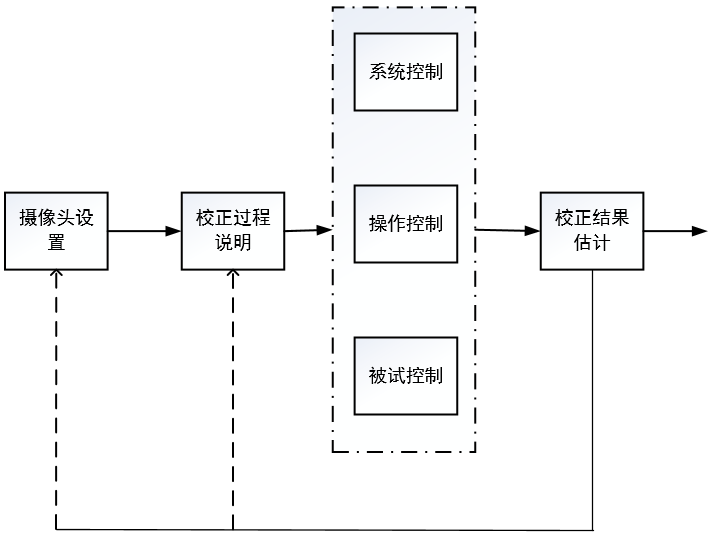
\includegraphics[width=0.6\textwidth]{chap1/calibrationprocess.png}
  \bicaption[fig:calibrationprocess]{眼动仪校正过程}{眼动仪校正过程}{Fig}{The eyetracker calibration process}
\end{figure}
各眼动仪厂家都会给出相应的校正方法\parencite{iview2009system,manual2011v3,manualuser}.

由于眼动仪厂家提供的校正方案只满足用户的基本需求,一些研究工作者对此做了更加精细的研究。迟健男等\parencite{chi2011sight}设计眼动仪时讨论了单摄像机、双摄像机以及多摄像机下的标定过程,最后采用了基于多摄像机全局标定的视线追踪系统来校准眼动仪,实验结果显示其水平误差为$1.5^{\circ}$ ,竖直误差为$1.9^{\circ}$ 。Marcus系统地研究了影响校正效果的各种因素\parencite{nystrom2013influence},包括不同的校正方法、被试者的眼睛生理特征、记录的时刻、注视的方向以及被试者的经验等,最后发现校正过程中提示用户观看目标比让用户自由观看目标效果好,甚至统计的结果还表明眼睛的颜色、睫毛、睫毛膏等也会影响数据的精度,因此,在我们后续的试验中需要避免这些干扰因素。Holmqvist给出了校正过程各个细节的注意事项\parencite{holmqvist2011eye},从目标的的设置、校正过程的操作、校正结果的验证等方面给出了详细的解决方案,这些方案对我们后面的工作具有很高的参考价值。

这些工作的目的是为了提升屏幕上视点的精度,它是为了满足2D场景下的精度要求设计的,这种方法被称为2D校正。由于人眼在屏幕上的注视点可以用左右眼的平均位置估计,所以当双眼误差方向相反时并不会影响最后估计的精度。但是在3D条件下,不仅需要单独估计双眼各自视点的精度,还要利用这两个点去计算双目视差角,所以,仅采用眼动仪自带的2D校准算法是不够的。Wang提出了一种3D校正算法\parencite{wang2014online},该算法在眼动仪原生的2D校正过程后执行。其核心思想是首先计算获得眼动数据的原始视差角,结合预设的视差角,采用拉格朗日最小方差的方法就可以获取系统偏差系数,从而利用该系数校准实验数据。Essig提出了一种叫做Parametrized Self-Organizing Map (PSOM)的方法\parencite{essig2006neural},该方法利用神经网络学习获取2D注视点到3D注视点的映射关系,然后从3D注视点获取深度信息。Pfeiffer在多个数据集上验证了普通的深度几何模型与PSOM的精度,得出了PSOM有更好效果的结论\parencite{pfeiffer2008evaluation}。这些方法在一定程度上提升了数据在3D意义下的精度,但是在实际使用中都有局限性,Wang的算法基于普通的深度几何模型,只适用于头部固定的眼动仪,而PSOM过于复杂,且时间效率不高。所以,在本文的前期工作中\parencite{ma2015new},对Wang的算法进行了改进,基本满足了精度与效率的要求。
\subsubsection{眼动数据滤波}
\label{chap1:sec:filter}
虽然不同公司生产的眼动仪略有差异,但是提供给用户的数据都比较类似。以Tobii眼动仪为例,用户可以获得实时的时间信息、屏幕上的注视点坐标、眼睛的位置坐标、双目距、瞳孔直径、眼动仪运行状态等信息。眼动数据处理的目的是获取人眼观看时的三种状态,即注视过程、扫视过程、眨眼等未知过程。因此传统的滤波方法是利用低通滤波器平滑眼动过程,然后采用聚类的算法分离眼动过程。Zhu提出了一种实时滤波的方法\parencite{zhu2002combining},首先利用Kalman滤波器追踪眼球,然后利用Mean Shift方法进行聚类。
Peng也做了类似的工作\parencite{peng2005mean}。Duchowski给出了眼动过程的分析方法\parencite{duchowski2007eye},深入讨论了信号去噪、注视点检测、扫视点检测等方法,这些方法为后续的研究做出了很重要的贡献。从工程实践的角度来看,Olsson为Tobii开发的滤波算法\parencite{olsson2007real}具有简单易实现、精度高的特点,其在忽略未知过程的基础上,可以将眼动数据分为注视过程与扫视过程,采用了中值滤波的方法消除高斯噪声,排除异常值的干扰。实验的结果显示,算法在精度与鲁棒性方面都有很高的水平。其他经典的算法还包括I-VT、1-HMM、I-DT、I-MST、I-AOI,Dario D. Salvucci对这些算法做了很好地总结与对比\parencite{salvucci2000identifying}。基于工程实践的考虑,本文的算法改进了Olsson的工作。

\subsubsection{眼动数据表示}
\label{eyetrackdatarepresentation}
获取眼动数据后,一般是以数据库或文本的形式保存,为了直观地观察眼动过程,眼动数据需要做可视化处理。目前最常见的眼动数据的表示方法有灰度图和伪彩色图两大类,前者以明暗程度来度量被注视的程度,后者则以色彩的鲜艳程度来表示,这一类图往往被称作注视密度图。注视密度图通常以高斯噪化的方法,将离散的注视点“模糊化”获取\parencite{wang2013computational}。通过直观地观察眼动数据,往往可以直接总结出眼动运动规律\parencite{kim2014saliency}。除了直观呈现以外,灰度图还可以作为眼睛注视程度的权重。Ulrich Engelke利用这种方法对比分析两个实验室不同被试者观看图片产生的注视密度图,发现即使在不同的实验室,采用不同的眼动仪,利用不同的被试者,其最终的结果在图像质量评价领域具有一致性\parencite{engelke2013comparative}。另外,国内学者也在眼动数据库的构建与可视化方面做出了相应的贡献\parencite{zhang2014dataset}。

这些方法在眼动数据的表示中发挥了很重要的作用,但是作为3D场景下的眼动数据,视差角信息是最重要的信息之一,上述方法无法反应视差角信息。如何表示3D场景下的眼动数据,我们提出了一种新的创建立体图像注视密度图的方法\parencite{ma2015new},更具体的过程将在第\ref{chap:dataprocess}章进行描述。
\subsection{眼动数据在2D图像质量评价中的应用}
\label{eyetrackapplied2D}
眼动数据真的可以提升图像质量评价效果吗?Ninassi对此提出了质疑\parencite{ninassi2007does},他结合了眼动数据的注视密度图和SSIM算法与MAD算法进行了验证,发现眼动数据对于JPEG和JPEG2000失真的图像并没有提升评价效果。但是,后面一系列的成果得出了相反的结论,Fliegel利用了眼动数据标注显著性区域\parencite{fliegel2008eyetracking},进而采用显著性区域的特征代替整体特征,结果发现,眼动数据的应用改进了评价效果。
Liu在这方面也做了大量的工作\parencite{alers2009using,liu2009studying,liu2011visual},其结果表明,无论是将眼动数据用于注视区域标注,还是将眼动数据用于模拟视觉注视过程,眼动数据都可以提升图像质量评价效果。Larson\parencite{larson2008can}利用了5个常见的图像质量评价方法,在两个眼动数据集上进行了验证,结果显示大多数评价方法在眼动数据的辅助下是可以提升评价效果的,更进一步,他们还发现,无任务的眼动数据采集要比有任务的采集效果更加明显。类似的工作还包括\parencite{gide2012comparative},
因此,当前学术界已经基本接受了眼动数据在图像质量评价中具有正面意义这一观点。总体来说,眼动数据在2D图像质量评价中的应用可以以图\ref{fig:eyetrackappliedin2D}来描述,\begin{figure}[ht]
  \centering
  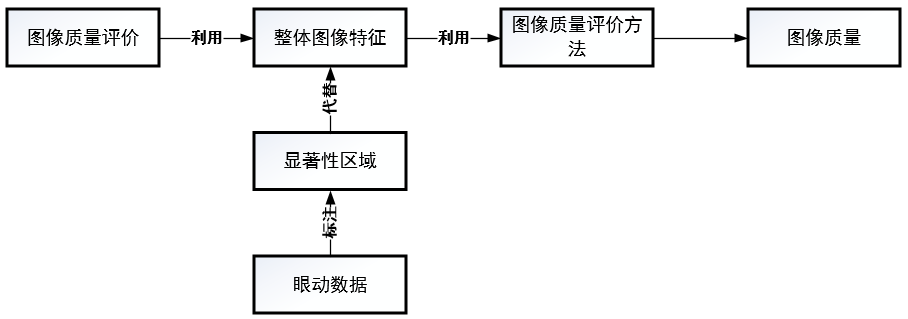
\includegraphics[width=\textwidth]{chap1/eyetrackerappliedin2dimage}
  \bicaption[fig:eyetrackappliedin2D]{眼动数据在2D图像质量评价中的应用方法}{眼动数据在2D图像质量评价中的应用方法}{Fig}{The application of eyetracking data in 2D image quality assessment}
\end{figure}

除了图像方面的应用,眼动数据在视频质量评价方面也发挥了重要的作用。Arndt针对空间域退化的视频,先后获取了眼动数据与脑电图,并以此建立了视频评价的方法\parencite{arndt2014using}。Jia利用眼动数据获取视频的显著性区域,提升了基于模糊和块效应的视频质量评价方法效果\parencite{jia2014no}。

眼动数据在图像/视频质量评价中除了直接获取显著性区域之外,还被作为显著性区域提取算法的ground truth。Yin给出了一种基于相位和幅度差异的视频显著性区域的检测算法,通过眼动数据验证了其精确度\parencite{yin2013video};张\parencite{zhang2013conside}则利用眼动数据验证了当前已有的显著性区域检测方法精度不高,提出了自己的显著性检测算法,并将其应用到了图像质量评价中。
\subsection{眼动数据在3D图像质量评价中的应用}
\label{sec:eyetrackapplied3D}
到目前为止,直接将眼动数据引入立体图像质量评价模型中的方法并不多见。眼动数据在3D图像质量评价方法中的应用与2D图像中的应用类似。第一,用于显著性区域的标注,然后将标注的区域用于立体图像质量评价\parencite{chung2004visual,wang2013computational};第二,用眼动数据验证显著性区域提取算法的精度。Wang利用2D+depth的思想来检测3D图像的显著性区域\parencite{wang2013computational},在提取图像的2D的显著性区域后,利用眼动仪提取了深度方向的显著性区域,二者的交集构成了新的显著性区域。结果表明,这比直接将2D显著性区域提取算法应用到3D图像中效果提升了很多。同时,该工作也贡献了一个3D眼动数据-立体图像库\footnote{ \url{http://ivc.univ-nantes.fr/en/databases/3D_Gaze/?article1103}}。Hanhart则建立了一个包括3D视频和主观评分的数据库\parencite{hanhart2014eyec3d},可以用来做视频质量评价。

值得注意的是,一些新的在立体图像中利用眼动数据的方法被提了出来。Kim利用眼动数据来验证了人眼对立体图像视差的反应过程,其结果表明人眼在低视差域可以很好地注视到显著性物体,相反地,在大视差域却不能\parencite{kim2014saliency}。Liu 的工作类似\parencite{liu2010dichotomy},他们发现人眼更喜欢注视亮度对比度和亮度梯度大的位置,而视差对比度和视差梯度比较大的位置则注视的比较少。这些工作不仅获得了有价值的结论,更重要的是其研究方法是挖掘眼动特征的重要工具。
\section{研究内容和结构安排}
\label{sec:arrangement}
随着人眼视觉模型在立体图像质量评价中发挥的作用越来越重要,眼动数据越来越被重视,除了用来标记人眼注视区域外,眼动数据本身的特征是否与立体图像质量相关就成为一个很有价值的研究问题。

本文的研究内容从立体图像-眼动数据库的创建开始,首先准备了实验所用的图像库,然后设计眼动实验,获取眼动数据。在此基础上,本文将给出3D场景下眼动数据的校正、滤波算法,并给出一种基于视差图分割的立体图像眼动注视密度分层表示方法,这些基础研究保证了眼动数据分析准确度以及合理性。有了这些基本的工具后,本文将处理眼动数据与主观评价数据,包括数据的去噪与异常测试剔除,然后会对眼动实验的结果进行分析。最后本文将基于前人成果和视觉生理过程等提取眼动数据特征,结合主观评分,利用SVR回归模型建立基于眼动数据的图像质量评价模型。

本文将包括六部分,具体安排如下:

第一章绪论,主要讨论课题研究的背景与意义。然后综述眼动数据处理技术,以及眼动数据在2D/3D 图像质量评价中的应用情况,最后对本文的工作做出安排。

第二章描述了人眼注视的生理过程,并以此分析了人眼生理过程与图像质量评价方法的联系。随后,针对我们的研究课题,描述了立体场景下的视差角,给出了眼动数据中视差角的计算方法。

第三章创建了立体图像-眼动实验库,首先选择了11幅内容有代表性的自然场景图像,然后通过视差调整获取了每幅图像的7种变换,最终得到了77幅用于实验的图像。然后设计了实验,实验包括主观评价实验和眼动实验,主观评分实验主要是成对比较实验,为了节约时间成本,将单刺激评分实验与眼动实验合并设计了有任务的眼动实验,眼动实验以眼动数据收集系统的开发开始,该系统既考虑了当前实验的需求,又考虑了以后其他方向的扩展,做好数据收集的准备。整个眼动实验包括三部分,立体视觉正常性检验,校正数据收集,带有主观评分的眼动数据收集等。这样便获取了研究所需素材。

第四章是数据分析,包括主观评分数据的分析与眼动数据的分析两部分,主观数据分析处理的目的主要是去除异常测试,并分析一些初步的实验结果。眼动数据处理则包括了眼动数据的3D校正、滤波以及可视化方法。眼动数据的3D校正过程利用3D眼动实验数据,获取每个被试者深度方向的偏差,并据此对立体图像观看下的眼动数据进行了系统性补偿。眼动数据的滤波过程对眼动数据进行了除噪以及眼动过程分离。眼动数据的可视化表示方法在立体图像分层的表示基础上,对眼动数据注视结果也进行了对应分层,形成了立体注视密度图。最终的实验结果表明以上处理技术是有效的。

第五章是眼动特征提取,眼动特征以前人的研究成果和视觉生理过程为基础来提出。眼动数据的静态特征根据人眼的注视结果提出,这里参考前人的研究成果\parencite{zhang2014application},本文从人眼的注视次数与时长、眨眼次数与时长等方面提取了一部分特征。眼动数据的动态特征则是根据人眼的运动过程来提出的。由于人眼在观看立体图像时视线会在不同区域跳变而产生不舒适感,因此,本文从跳变的幅度,次数等方面提取了一部分特征。视差信息是立体图像的重要信息之一,也是影响图像质量的重要因素,人眼观看立体图像过程中存在深度调整——辐辏调节,这是产生视觉疲劳的重要原因,因此本文从视差角的角度出发提取了一部分特征。然后基于SVR对特征集与主观评分建模,观察并分析了模型结果。

第六章为总结与展望,对本课题的研究内容进行了回顾与总结,并提出可以改进的地方和可能的研究方向。

